%\documentclass[final,3p]{article}
\documentclass[final,12p]{article}
\usepackage{graphicx}
\usepackage[letterpaper,margin=1.0in]{geometry}
\usepackage{amssymb}
\usepackage{changepage}
\usepackage{float}
\usepackage{hyperref}
\usepackage{url}
\usepackage{afterpage}
\usepackage{natbib}
\usepackage{setspace}
\usepackage{fancyhdr}
\pagestyle{fancy}
\fancyhf{}
\usepackage[utf8]{inputenc} 
\usepackage{lastpage}

\def\Student{Ashish Sehrawat}
\def\Title{THESIS PROJECT PROPOSAL}
\def\Prog{Doctorado en Ciencias (F\'{i}sica) }
\def\Dept{Departamento de Investigac\'{i}on en Fis\'{i}ca}
\def\Institution{Universidad de Sonora}
\def\Director{Dr. Jos\'{e} Feliciano Ben\'{i}tez Rubio}
\def\ProjectTitle{Measurement of the luminosity in proton-proton collisions at the CMS experiment of the Large Hadron Collider}
\def\ResearchLine{Astrof\'{i}sica, Cosmolog\'{i}a y F\'{i}sica de Part\'{i}culas}

%%header and footer
\lhead{\Student\ / \ \Dept}
\rhead{\Title}
\rfoot{Page \thepage \hspace{1pt} of \pageref{LastPage}}


%%%%%%%comands
\newcommand{\SubItem}[1]{ {\setlength\itemindent{15pt} \item[-] #1} }
\newcommand{\lumi}[1]{{#1~fb$^{-1}$}}
\newcommand{\instlumi}[1]{#1$\times 10^{34}$ cm$^{-2}$s$^{-1}$} }

  

%%%%%%%%%%%%%%%%%%%%%%%%%%%%%%%%%%%%%
\begin{document}
\onehalfspacing

%%%%Title Page
\begin{titlepage}
\centering
\hspace{0pt}
\vfill
{\scshape\Large \Title \par}
project revised 2021-1
  
  \vspace{2cm}
  {
    TITLE:\par
    {\bf \large \ProjectTitle \par}
  }
       
  \vspace{0.5cm}
  {
    RESEARCH LINE: \par
    \ResearchLine \par
  }
        
  \vspace{4cm}
  {\underline{\hspace{8cm}}\par}
  {\bf \scshape \Student \par}
  {Student\par}

  \vspace{1cm}
  {\underline{\hspace{8cm}}\par}
  {\scshape \Director \par}
  {Director\par}

  \vspace{1cm}
  {\bf \Prog \par}
  {\Dept \par}
  {\Institution \par}

  \vspace{4cm}
  {\today}

\hspace{0pt}
\vfill

\end{titlepage}


%%%%% white page for print out
\shipout\null


%%%% Abstract Page
\newpage
\hspace{2pt}
\vfill

  \begin{center}
    {\Large \ProjectTitle \par}
    \vspace{1cm}
    {\itshape\textbf{Abstract}\par}
  \end{center}
  
  \vspace{1 cm}
 
  
  This research project proposes to determine precise value and corresponding uncertainity of luminosity delivered to Compact Muon Solenoid (CMS) experiment at CERN during 2017-2018 period using Pixel Cluster Counting (PCC) method and construction of luminosity measurement device using Tracker Endcap Pixel Detector (TEPX) for High Luminosity (HL)-LHC which will be able to withstand luminosities of up to 3000 $fb^{-1}$. Luminosity plays a vital role in determination of cross section for various production and decay processes of elementary particles and its accurate determination will assist in precise calculation of SM quantities like cross section, couplings and exploring physics beyond SM.     

  \hspace{2pt}
\vfill



%%%%%% Begin the body
\newpage
\section{BACKGROUND}


The standard model (SM) of particle physics is so far the best theoretical model to describe the interaction of elementary particles mediated by three of the four fundamental forces of nature which are electromagnetic force, strong nuclear force and the weak nuclear force. The SM is divided into two categories, the bosonic sector and the fermionic sector.
The bosonic sector contains particles which mediate the fundamental forces of nature and the fermionic sector contains particles which make up all known matter in our universe.
There are three generations of fermion particles: the first generation consists of up (u) quark, down (d) quark, electron and electron neutrino, the second generation consist of charm (c) quark, strange (s) quark, muon and muon neutrino, and the third generation has the top (t) quark, bottom (b) quark, tau and tau neutrino.
The bosonic sector consists of the gauge bosons: gluon, photon, $W^{\pm}$, $Z^0$ which mediate strong nuclear force, electromagnetic force and weak nuclear force respectively.
The Higgs boson ($H$), is the last of the gauge bosons, it gives mass to the other SM particles via electroweak symmetry breaking mechanism \cite{Chatrchyan:2012xdj}.
The heavy particles ($W^{\pm}$, $Z^0$, $H$, and top) can only be produced at high energy particle colliders like the Large Hadron Collider (LHC) operating at a center-of-mass energy of 13 TeV in Geneva, Switzerland.
Until the 90s, existence of almost all the SM particles were confirmed except the top quark and the Higgs boson. 
These had eluded previous experiments due to difficulties in the production and reconstruction of its decay products.
The top quark was discovered in 1995 at the Tevatron collider of the Fermilab laboratory, this proton collider operated with a center-of-mass energy of 1.8 TeV until 2010.
In 2012, the ATLAS and CMS experiments, with detectors placed at two points where the proton beams collide in the LHC, announced the discovery of a new particle with a mass of 125 GeV.
This particle has been identified as the Higgs boson by measuring its properties and comparing to those predicted by the SM.


Luminosity, $L$, is a key parameter at particle colliders along with the energy available in the collision.
$L$ is one of the  main figures of merit that quantify the potential for observing new particles and measuring their properties.
The instantaneous luminosity $L(t)$ is the process-independent ratio between the rate $R(t)$ of events produced per unit time and the cross section for a given process $\sigma$: $L(t) = R(t)/\sigma$.
During Run 1 (2011-2012) LHC reached a peak instantaneous luminosity of \instlumi{0.77} and delivered an integrated luminosity of about \lumi{25} with a precision of about 2.0\% 
\footnote{1 barn is a unit of area corresponding to $10^{-24}$ cm${^2}$ and 1 femtobarn (fb) = $10^{-39}$ cm$^{2}$. For comparison, the total Higgs production cross section is 48600 fb.}.
In the first part of Run 2 (2015-2016), the delivered luminosity has been measured to be \lumi{38.4} with an unprecedented precision of 1.3\% \cite{Sirunyan:2021qkt}.
For the second part of Run 2 (2017-2018), the integrated luminosity is about \lumi{78}, but its precise value and uncertainty remain to be determined and is one of the main objectives of this thesis project \cite{CMS:2018elu}.

The plan of the LHC till year 2038 is to obtain datasets with up to 10 times higher values of instanteneous luminosities in the final phase, the  High Luminosity LHC (HL-LHC), and corresponding integrated luminosities of order \lumi{3000} as shown in Figure~\ref{figure6}.
These final datasets will provide  precise measurements of the properties of the Higgs boson and other SM particles as shown in Fig. ~\ref{figureKappasUncs}.
This figure shows that one of the dominant uncertainties which remain to be determined is due to the luminosity measurement.
In this project, we also perform studies for the design and construction of an upgraded luminosity measurement system to be installed for CMS in the HL-LHC phase}\cite{Collaboration:2706512}.



\begin{figure}[H]
  \centering
  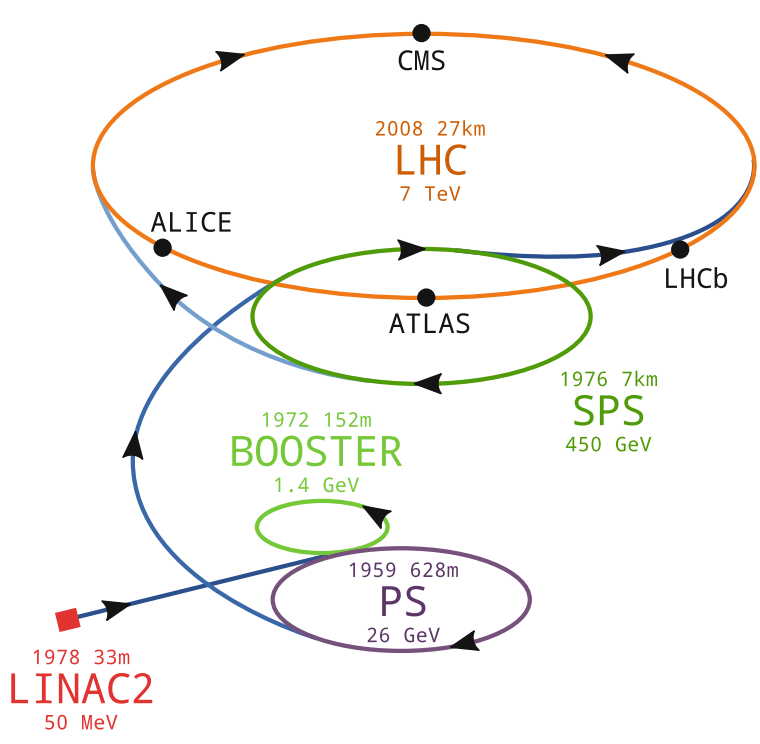
\includegraphics[width=0.7\columnwidth]{./LHCcomplex.png}
  \caption{Diagram of the LHC accelerator complex located near Geneva, Switzerland. The complex consists of three accelerator stages: the proton (p) or lead (Pb) source, the Proton Synchrotron (PS), the Super Proton Synchrotron (SPS), and the 27 km LHC ring. Four collision points are shown corresponding to the ALICE, ATLAS, LHCb, and CMS detectors  \cite{Mobs:2684277}. }
  \label{figure5}
\end{figure}


\begin{figure}[H]
  \centering
  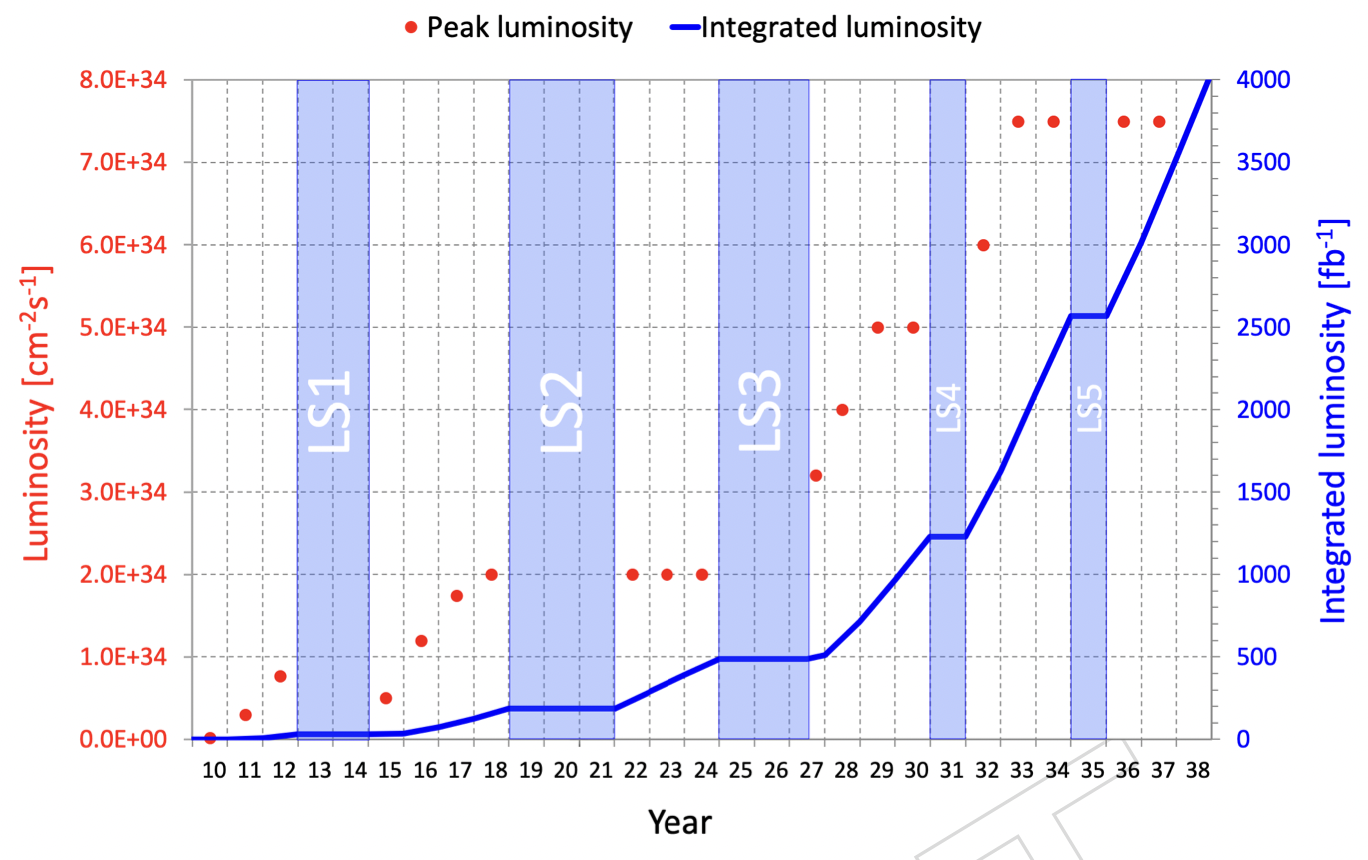
\includegraphics[width=0.8\columnwidth]{./HLLHCLumi.png}
  \caption{Projected performance of the LHC until 2038, which shows the preliminary dates for prolonged stops (LS) of the LHC and luminosities. Points show instantaneous luminosity while the line shows luminosity accumulated \cite{collaborations2019report}.}
  \label{figure6}
\end{figure}


 \begin{figure}[H]
   \centering
   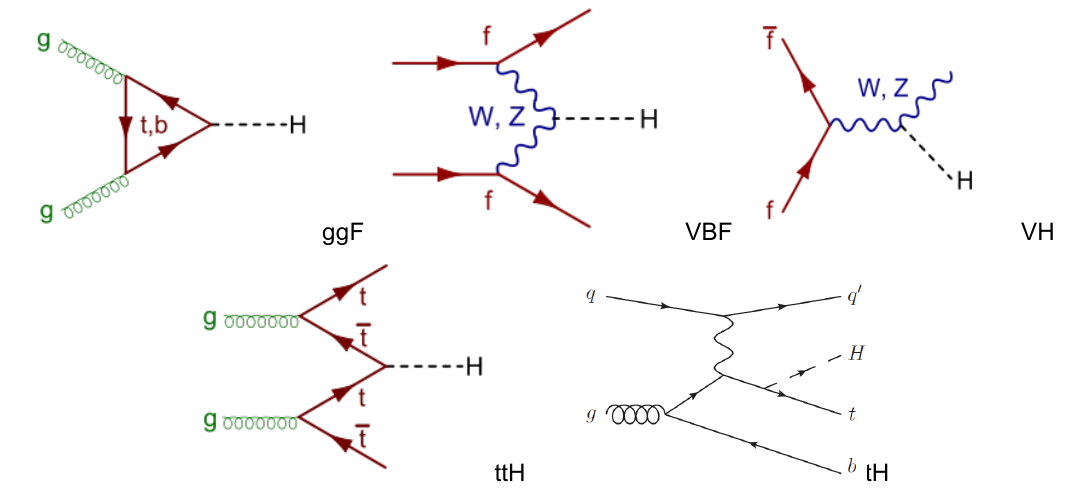
\includegraphics[width=0.7\columnwidth]{./pg.png}
   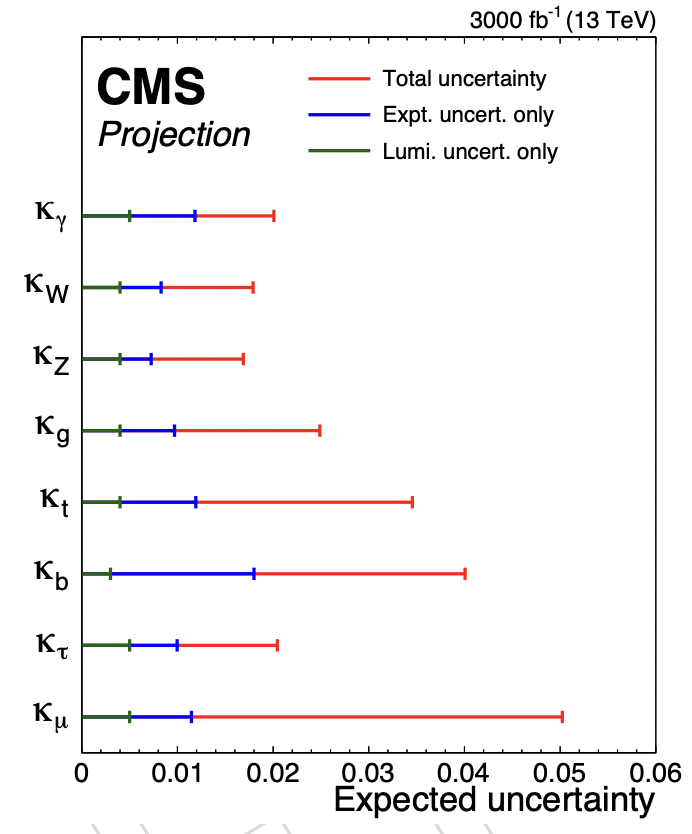
\includegraphics[width=0.29\columnwidth]{./higgs_couplings.png}
   \caption{
     Left: Main production mechanisms for the Higgs boson at the LHC: gluon-gluon fusion (ggF), vector-boson fusion (VBF), associated vector boson (VH), associated top-quark pair (ttH), and  associated single-top quark production (tH)  \cite{Grojean:2017hsb}  \cite{Khachatryan:2015ota} .
     Right: Expected uncertainties on the Higgs coupling parameters for  \lumi{3000} of proton-proton collision data at 13 TeV center-of-mass energy \cite{Cepeda:2019klc}.
   }
   \label{figureKappasUncs}
 \end{figure}




\section{PROPOSAL}

This project has two main parts, in the first part we propose to perform an analysis of the LHC luminosity data  recorded by the CMS experiment during 2017 and 2018 using Pixel Cluster Counting (PCC) method.
In the second part we develop an upgraded luminosity measurement system for the HL-LHC phase (2026-2038).

\section{GENERAL OBJECTIVE}

The main objective of this work is to perform a measurement of the 2017-2018 LHC delivered luminosity with a precision at the level of 2\% or less using the CMS Pixel detector.
This precision is necesary for testing SM of elementary particles and identifying possible new physics which could elucidate the nature of Dark Matter in our universe. 

The second objective is to develop an upgraded luminosity measurement system for the HL-LHC phase using Tracker Endcap Pixel detector (TEPX). TEPX is a part of new tracker detector proposed by the CMS collaboration which will replace the current one during LS3 (2024-2026). 

\section{HYPOTHESIS}

As mentioned in the introduction, precision achieved in the measurement of integrated luminosity during Run 1 was about 2.5\% using  methods developed for the first time.
In 2015 and 2016 the uncertainty achieved was 1.6\% and 1.2\%, respectively, for datasets corresponding to \lumi{2.5} and \lumi{36}  \cite{Sirunyan:2021qkt}.
The methods used for the 2015 and 2016 data are similar to the strategy we propose in this project.
We expect that the final uncertainties for the 2017 and 2018 datasets to be similar, but the ultimate goal of the CMS collaboration is to reduce these uncertainties to below 1\%  \cite{Dainese:2019rgk}.

For the upgrade part of this project, we must consider that in the HL-LHC phase the higher expected pileup (number of proton collisions per bunch crossing) will lead to more difficult scenarios for the luminosity measurement due to increased detector occupancy and larger irradiation of the detector components. 
However, we expect that new methods to be introduced between now and the start of the HL-LHC phase will improve the measurement precision and compensate the higher backgrounds and detector aging.  


\section{SPECIFIC OBJECTIVES}

For the Run 2 luminosity measurement:
\begin{itemize}
\item understand the CMS pixel detector layout including the barrel layers and endcap disks and their constituent modules,
\item study the stability of the modules in the different layers or disks of the pixel detector and select the stable components,
\item calculate the visible cross section corresponding to the PCC rate for proton-proton colisions at 13 TeV using the selected pixel detector components,
\item study the stability and linearity of the PCC luminosity measurement by comparing to other CMS luminometers as a measurement of the systematic uncertainties,
\item determine the delivered luminosity per lumisection (23 second intervals) and the total integrated luminosity and determine the corresponding uncertainty.
\end{itemize}

\par
For the development of the HL-LHC upgrade system:
\begin{itemize}
\item study the different parts of the TEPX detector.
\item study the pixel cluster counting at the HL-LHC conditions using simulations of the TEPX detector.
\item develop an algorithm for counting cluster coincidences using sensor layers of the same disk in the TEPX detector in order to reduce backgrounds.
\item determine the linearity and statistical precision of the PCC method and coincidence counting method for the TEPX detector and its constituent parts (disks and rings).
\end{itemize}


\section{METHODOLOGY}


The CMS experiment is located at one of the four interaction points of LHC.
The CMS detector has the form of a cylindrical onion, with several concentric layers of components.
A powerful magnet is used to bend charged particles as they move away from the point of collision to identify the charge and measure their momentum.
A silicon tracker, made of about 75 million electronic sensors arranged in concentric layers, measures the curvature of charged particles with very high precision \cite{Chatrchyan:2008aa}.
The electromagnetic calorimeter detects photons and electrons while the hadron calorimeter detects mainly pions and kaons.
The muons are detected by special chambers placed outside the solenoid as shown in Figure~\ref{fig:CMS}.

The PCC method for measuring luminosity uses the Pixel detector of the CMS tracker, the layout of the  detector used for recording the data during 2016-2018 is shown in Figure~\ref{fig:pixeldet}.
The Pixel detector consists of 4 concentric cylindrical layers in the barrel and 2 disks in each endcap.
Each detector part is composed of pixel sensors, a schematic of one sensor is shown in Figure~\ref{fig:pixeldet}.
The entire Pixel detector contains 1856 sensor modules and a total of 65 million pixels.

The PCC method consists of the reconstruction of track clusters produced by charged particle tracks as shown in Figure~\ref{fig:trackcluster}.
Due to the fine granularity of the pixel sensors and the large number of total pixels, the hit occupancy in the sensors remains very small, order of 1\%, during normal collisions.
This low occupancy makes the PCC  very linear as a function of pileup, an essential property of a good luminometer.

The calibration of the luminometer consists of a van der Meer (vdM) scan performed in a special LHC run usually at the beginning of the run period (year).
In this calibration setup, proton beams are moved across each other in separation steps of about 100 micrometers, by measuring the rates of clusters with the PCC algorithm and knowledge of the beam parameters during the vdM conditions, the calibration constant ($\sigma_{vis}$) is determined.
This calibration constant is then used to normalize the measured PCC rates during normal running throughout the data-taking year.

For the upgrade part of this project, the research consists of studying the expected performance of the TEPX disks of the CMS tracker in the HL-LHC phase.
The current design of the this tracker is shown in Figure~\ref{fig:tepx}, where the TEPX part consists of the last 4 disks at $|z|>170$ cm. In the same figure a transverse view of one disk is shown, and shows the layout of the sensor modules along phi for each ring in the disk.
Studies will be performed using simulated samples with HL-LHC beam conditions, currently the expected pileup for these conditions is about 200 proton collisions per bunch crossing.
The linearity of the cluster counting algorithm will be studied.
In addition, a new algorithm will be developed to detect cluster coincidences between consecutive layers of a disk.
It is expected that coincidences will be less sensitive to backgrounds in HL-LHC pileup conditions and therefore a more robust luminosity measurement can be performed.


\begin{figure}[H]
  \centering
  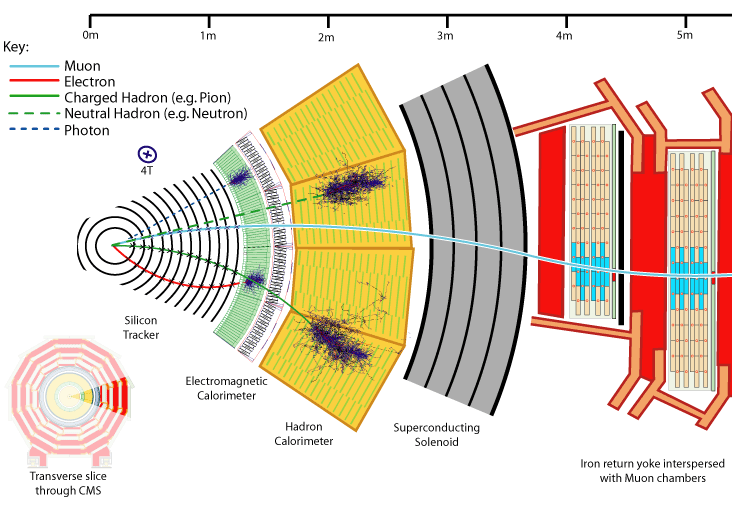
\includegraphics[width=0.7\columnwidth]{./cms12.png}
  \caption{Transverse view of the CMS detector showing the silicon tracker, electromagnetic calorimeter, hadron calorimeter, superconducting solenoid and muon chambers \cite{Chatrchyan:2008aa}.}
  \label{fig:CMS}
\end{figure}

\begin{figure}[H]
  \centering
  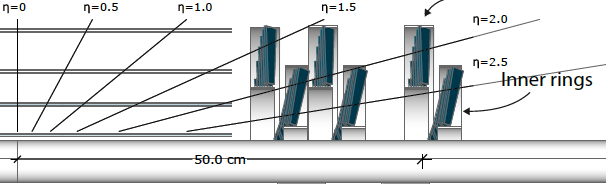
\includegraphics[width=0.7\columnwidth]{./PixelDetectorPhase1.png}
  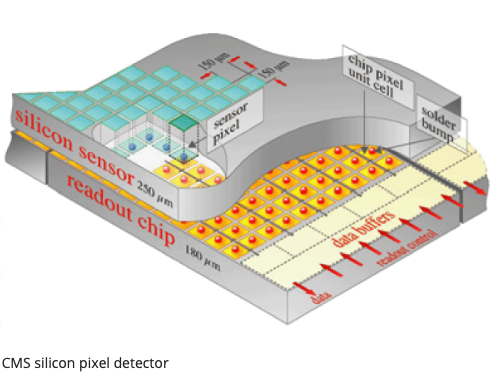
\includegraphics[width=0.27\columnwidth]{./PixelSensor.png}
  \caption{
    Left: diagram showing the layout of the CMS Pixel detector used during 2016-2018.
    The layout consists of 4 barrel layers and 2 endcap disks with two rings each.
    Right: a diagram showing the structure of one pixel sensor.
    The entire detector consists of 1856 sensors and 65 million pixels \cite{TrackerGroupoftheCMS:2020bgg}.
  }
  \label{fig:pixeldet}
\end{figure}

\begin{figure}[H]
  \centering
  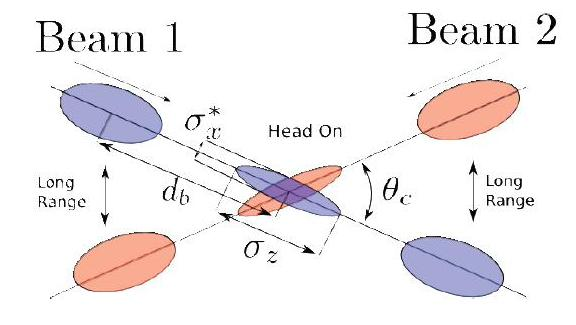
\includegraphics[width=0.5\columnwidth]{./bunchcrossing.jpg}
  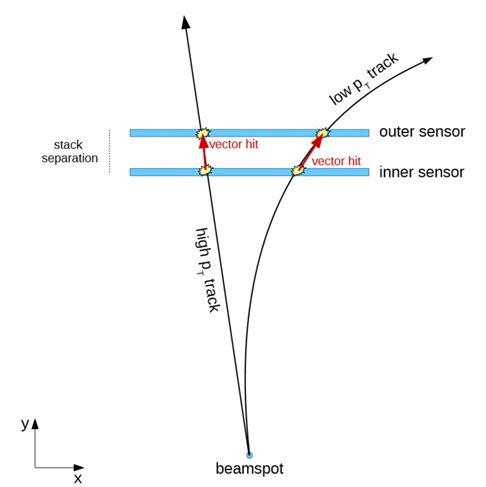
\includegraphics[width=0.4\columnwidth]{./vectorhit1.jpg}
  \caption{
    Left: Diagram showing the collision of two proton bunches at LHC, bunches contain about $10^{11}$ protons  \cite{deMaria:2008zzb}.
    Right: diagram showing example tracks originating from the collision at the beamspot and producing clusters at the pixel sensors in two detector layers.
  }
  \label{fig:trackcluster}
\end{figure}



\begin{figure}[H]
  \centering
  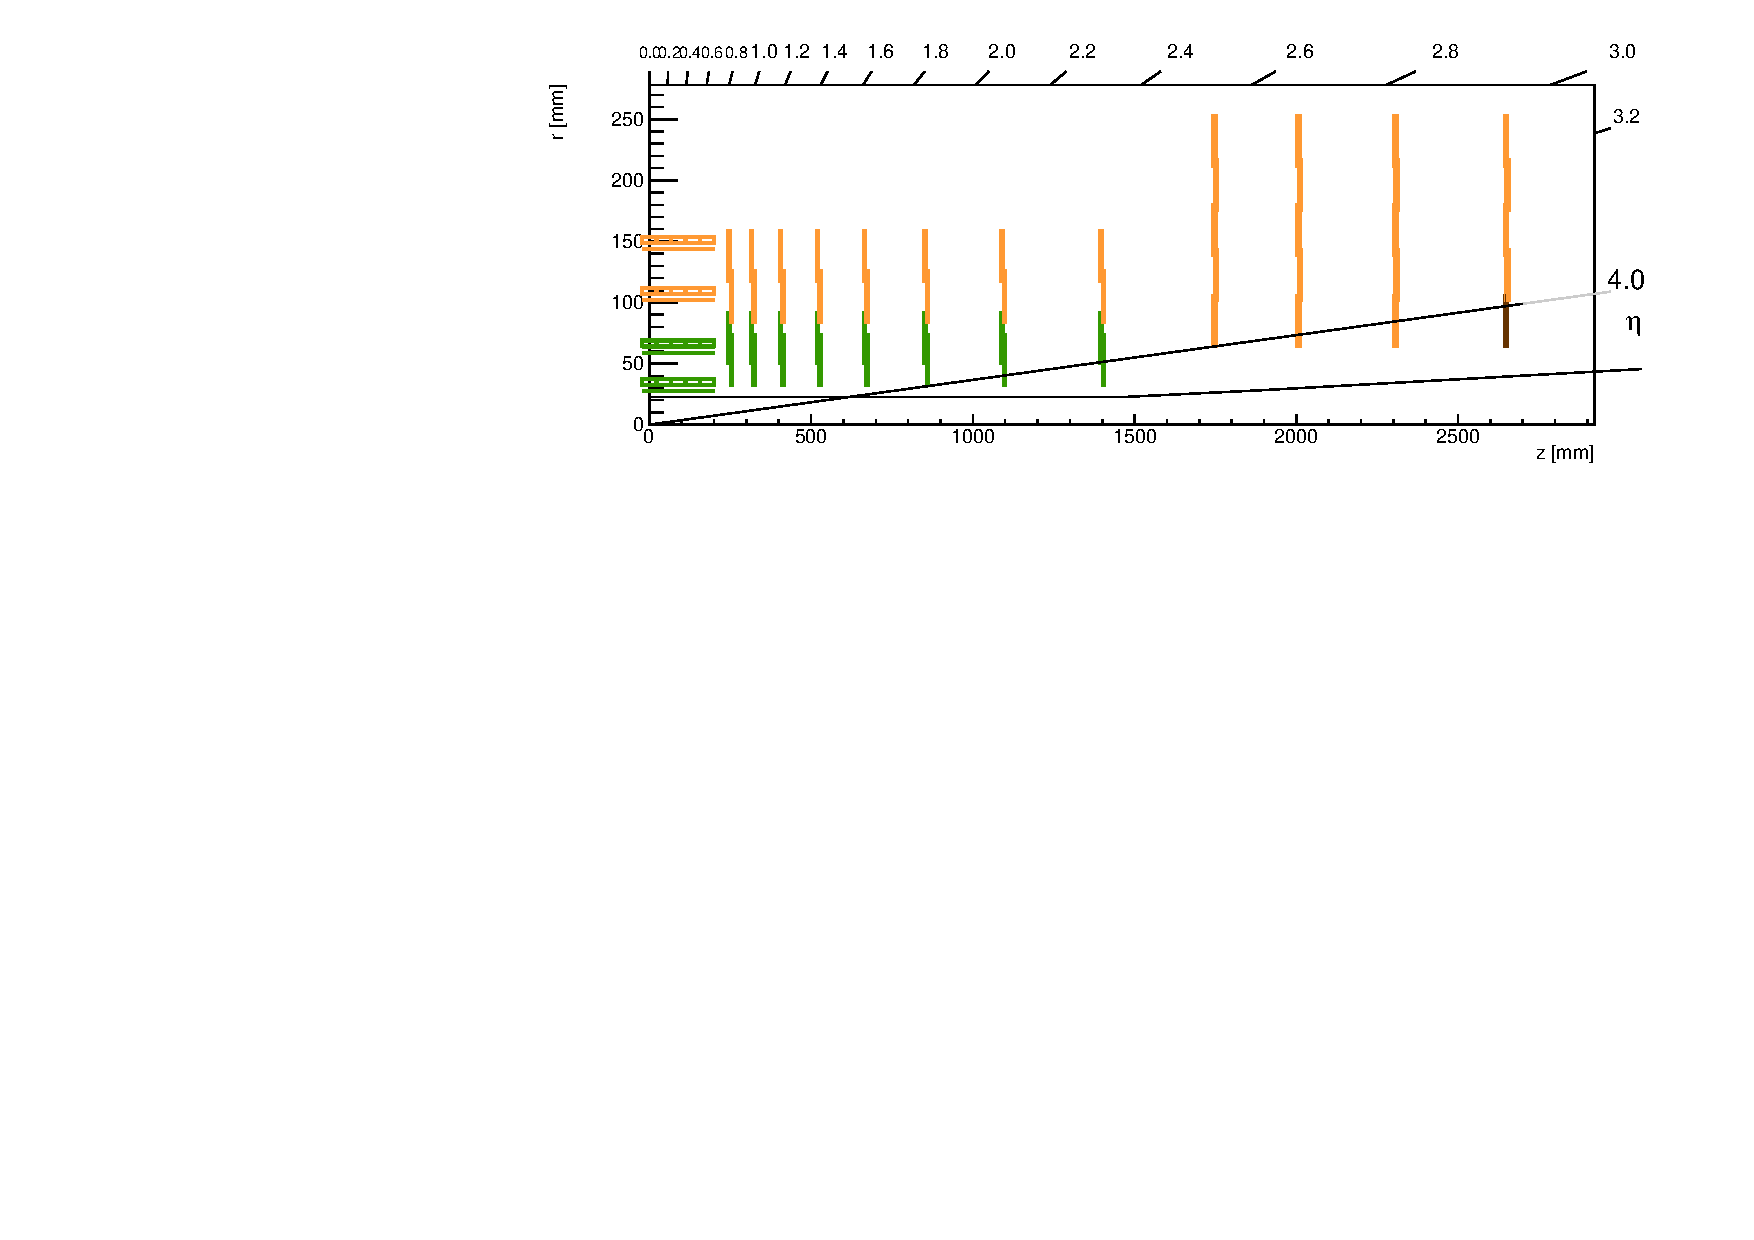
\includegraphics[width=0.7\columnwidth]{./TEPX_rz.pdf}
  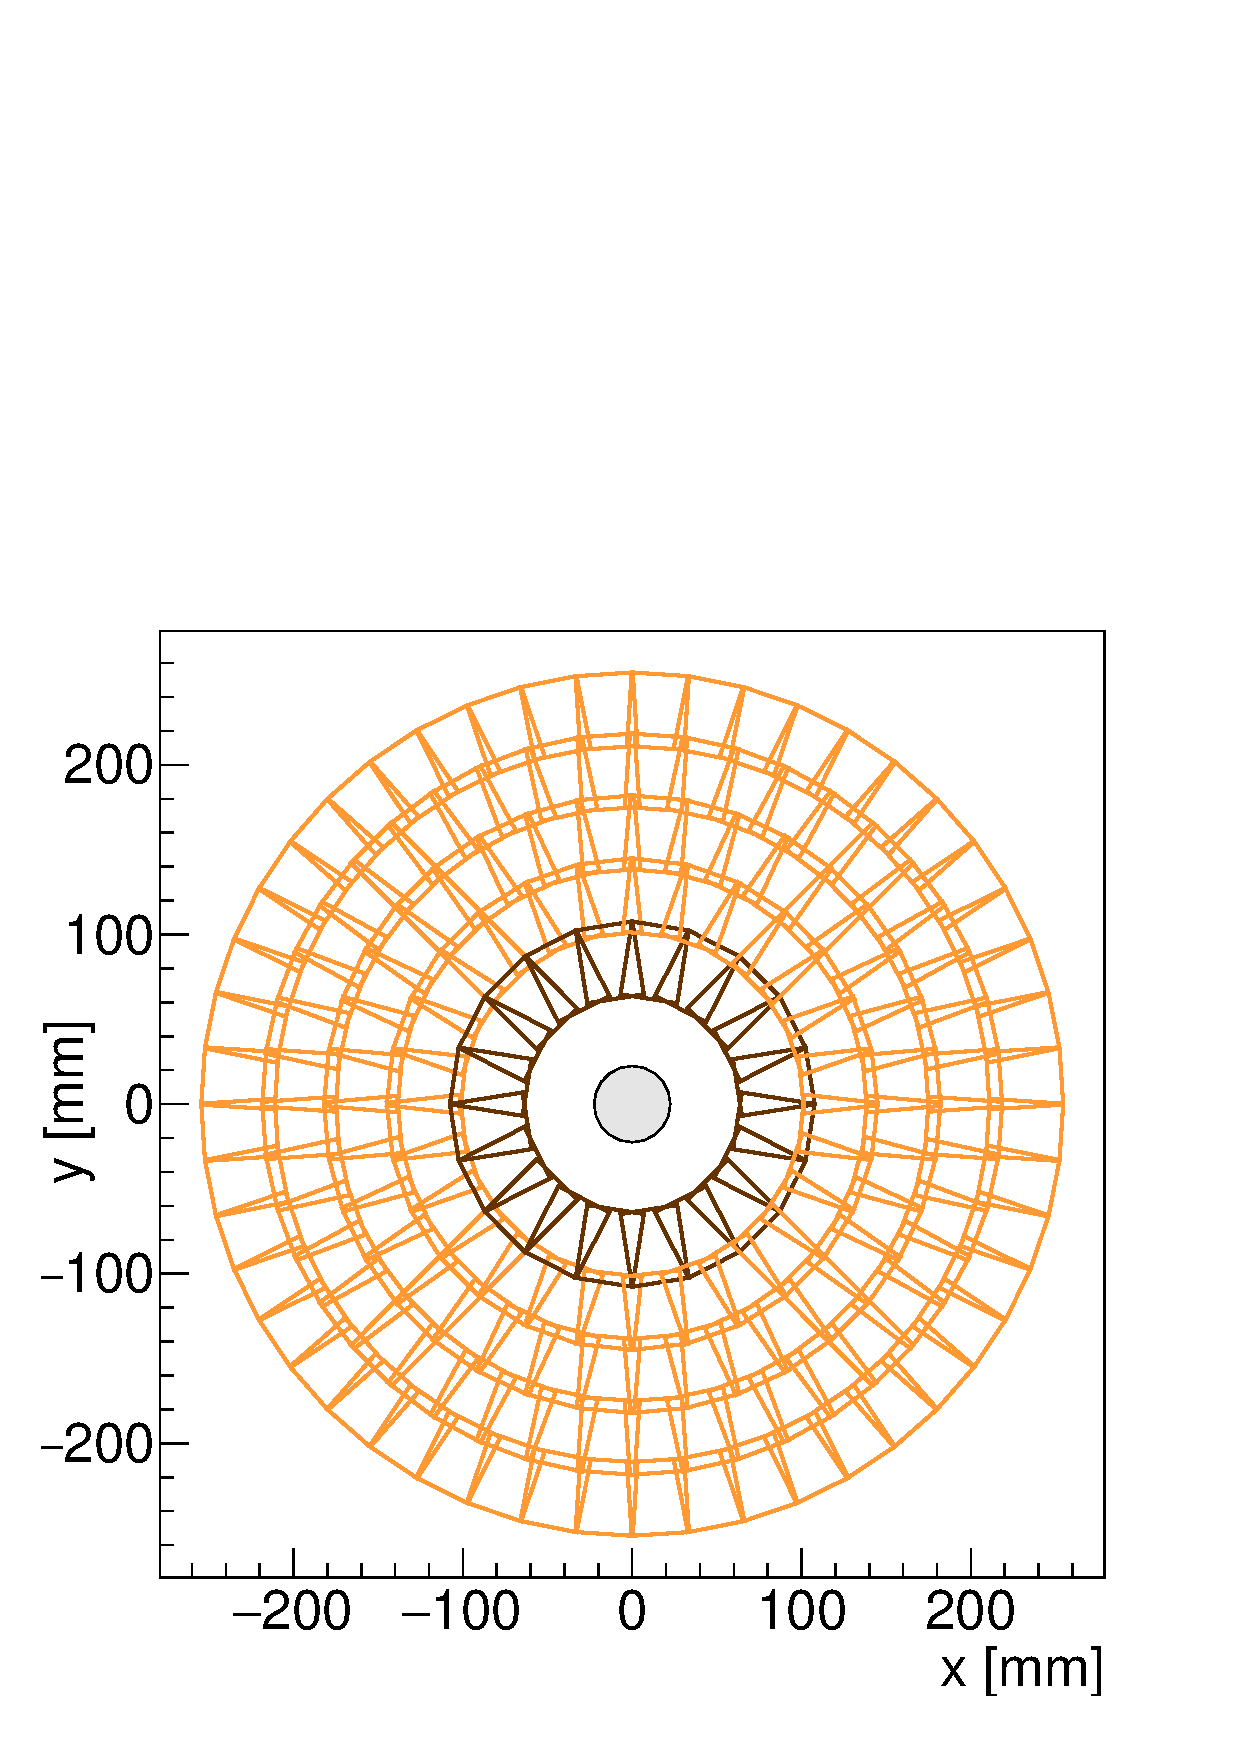
\includegraphics[width=0.27\columnwidth]{./TEPX_rphi.pdf}
  \caption{
    Left: Longitudial view of the current design of the CMS tracker detector for the HL-LHC phase. The TEPX consists of the last 4 disks on each side at $|z|>$ 1700 mm.
    Right: Transverse view of one TEPX disk showing the layout of the sensors in each of the 5 rings \cite{Klein:2017nke}.
  }
  \label{fig:tepx}
\end{figure}




\section{EXPECTED RESULTS}

From this project two main publications are expected:
\begin{itemize}
\item
For the Run 2 luminosity mesurement, the student will perform the studies for the selection of good modules for calculating luminosity using the PCC method.
From past performance of this algorithm it is expected that this measurement will give one of the best linearity and stability systematic uncertainties for the integrated luminosity value.
The results of these studies will be published in a peer-reviewed scientific journal.
\item
For the development of the HL-LHC upgrade system, we expect to produce a Technical Design Report (TDR) with the proposed design and algorithms to use the TEPX detector. This document will be published in the CERN document server (CDS) and submitted to the LHC committee for approval of required funding for the construction and operation of the system.
\end{itemize}

Also, the student will become a part of an international experiment and is expected to present his results at national or international scientific conferences.



\section{CALENDAR OF ACTIVITIES}

\begin{itemize}

\item {\bf Semester 1 (2019-2)}:
  \SubItem{ Readings on Standard Model of particle physics theory}
  \SubItem{ Basic Linux computing skills (\textsc{Bash, Emacs, Root})}
  \SubItem{ Initial planning of the analysis strategy}

\item {\bf Semester 2 (2020-1)}:
  \SubItem{ Course I on particle physics, particle detection, or data analysis}
  \SubItem{ Readings on the LHC and CMS experiments}
  \SubItem{ Basic Linux computing skills (\textsc{Bash, Emacs, Root})}
  \SubItem{ Computing accounts at CERN and Fermilab}
  \SubItem{ Studies of the TEPX luminometer upgrade}

\item {\bf Semester 3 (2020-2)}:
  \SubItem{ Course II on particle physics, particle detection, or  data analysis}
  \SubItem{ Studies of the TEPX luminometer upgrade}

\item {\bf Semester 4 (2021-1)}:
  \SubItem{ Completion of the TEPX luminometer studies for the TDR document}
  \SubItem{ Studies of the LHC Run 2 data using the PCC method}
  \SubItem{ Writing of the monograph}

\item {\bf Semester 5 (2021-2)}:
  \SubItem{ Publication of the TDR document in CDS and submission to the LHCC for review}
  \SubItem{ Presentation at national or international conferences of the TEPX upgrade studies}
  \SubItem{ Studies of the LHC Run 2 data using the PCC method}
  
\item {\bf Semester 6 (2022-1)}:
  \SubItem{ Completion of the studies of the Run 2 data luminosity measurement}
  \SubItem{ Writing of the Run 2 data luminosity measurement publication and review within the CMS collaboration}

\item {\bf Semester 7 (2022-2)}:
  \SubItem{ Publication of the Run 2 data luminosity measurement in a peer reviewed journal}

\item {\bf Semester 8 (2023-1)}: 
  \SubItem{ Presentations at national or international conferences for both the Run 2 luminosity measurement and TEPX luminometer for HL-LHC}
  \SubItem{ Writing of the Ph.D thesis}
  
\end{itemize}


\onehalfspacing
\bibliographystyle{unsrt}
\bibliography{paper}

\end{document}

